% Overview of bsky-manifold-arb (Bluesky -> Manifold auto-trader).
% Written against src/ (main, ingest, extract, sieve, pipeline, triage,
% belief, trade, discord, onboarding) and docs/SPEC.md + docs/HANDOFF.md.
% Compile: pdflatex OVERVIEW.tex
\documentclass[10pt,a4paper]{article}
\usepackage[margin=1.8cm]{geometry}
\usepackage{tikz}
\usetikzlibrary{positioning,arrows.meta}
\usepackage{amsmath}
\usepackage{booktabs}
\usepackage{array}
\usepackage{enumitem}
\usepackage[hidelinks]{hyperref}
\usepackage{titlesec}

% Compact spacing to fit two pages.
\setlength{\parindent}{0pt}
\setlength{\parskip}{3pt}
\titlespacing*{\section}{0pt}{7pt plus 2pt minus 1pt}{3pt}
\titlespacing*{\subsection}{0pt}{5pt plus 1pt minus 1pt}{2pt}
\titleformat{\section}{\large\bfseries}{\thesection}{0.6em}{}
\titleformat{\subsection}{\normalsize\bfseries}{\thesubsection}{0.6em}{}

\newcommand{\pint}{p_{\mathrm{int}}}
\newcommand{\pmkt}{p_{\mathrm{mkt}}}
\newcommand{\logit}{\operatorname{logit}}

\begin{document}

\begin{center}
  {\LARGE\bfseries bsky-manifold-arb}\\[3pt]
  {\large A Bluesky $\to$ Manifold auto-trader --- how it works}\\[3pt]
  {\small One Rust binary, one tokio runtime, one SQLite database. The value is \emph{filtering}: turn the Bluesky firehose into a handful of ``this matters for market $X$'' posts, and trade only on strong edge. Discord is the only control plane.}
\end{center}

\section{Big picture}\label{sec:big}

The bot streams the Bluesky \textbf{Jetstream} firehose, cheaply filters every
post through one compiled \textbf{Sieve} rule per tracked market (plus a VIP
author bypass), and only for survivors calls \emph{one small LLM} via Cloudflare
Workers AI. A material post nudges a per-market log-odds belief; the belief is
compared to the live Manifold price, and a fractional-Kelly trade is placed only
when the gap is wide. Each market has an isolated mana budget.

\begin{center}
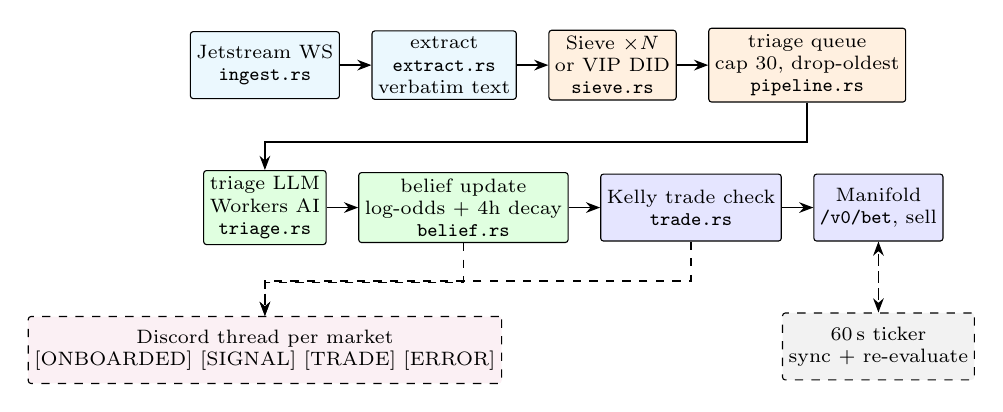
\begin{tikzpicture}[
  box/.style={draw, rounded corners=1pt, align=center, font=\scriptsize,
              inner sep=2.2pt, minimum height=8.5mm},
  arr/.style={-{Stealth[length=1.8mm]}, semithick},
  every node/.append style={font=\scriptsize}
]
% Row 1 (top): ingestion -> matching -> queuing.
\node[box, fill=cyan!8]   (n1) {Jetstream WS\\\texttt{ingest.rs}};
\node[box, right=4mm of n1, fill=cyan!8] (n2) {extract\\\texttt{extract.rs}\\verbatim text};
\node[box, right=4mm of n2, fill=orange!12] (n3) {Sieve $\times N$\\or VIP DID\\\texttt{sieve.rs}};
\node[box, right=4mm of n3, fill=orange!12] (n4) {triage queue\\cap 30, drop-oldest\\\texttt{pipeline.rs}};
% Row 2 (bottom): LLM -> belief -> trade -> Manifold.
\node[box, below=9mm of n1, fill=green!12] (n5) {triage LLM\\Workers AI\\\texttt{triage.rs}};
\node[box, right=4mm of n5, fill=green!12] (n6) {belief update\\log-odds + 4h decay\\\texttt{belief.rs}};
\node[box, right=4mm of n6, fill=blue!10] (n7) {Kelly trade check\\\texttt{trade.rs}};
\node[box, right=4mm of n7, fill=blue!10] (n8) {Manifold\\\texttt{/v0/bet}, sell};
% Events side-channel.
\node[box, below=9mm of n5, fill=purple!6, dashed] (n9) {Discord thread per market\\{[ONBOARDED] [SIGNAL] [TRADE] [ERROR]}};
\node[box, below=9mm of n8, fill=gray!10, dashed] (n10) {60\,s ticker\\sync + re-evaluate};

\draw[arr] (n1) -- (n2);
\draw[arr] (n2) -- (n3);
\draw[arr] (n3) -- (n4);
\draw[arr] (n4.south) -- ++(0,-5mm) -| (n5.north);
\draw[arr] (n5) -- (n6);
\draw[arr] (n6) -- (n7);
\draw[arr] (n7) -- (n8);
\draw[arr, dashed] (n6.south) -- ++(0,-5mm) -| (n9.north);
\draw[arr, dashed] (n7.south) -- ++(0,-5mm) -| (n9.north);
\draw[arr, dashed] (n8.south) -- ++(0,-5mm) -| (n10.north);
\draw[arr, dashed] (n10.north) -- (n8.south);
\end{tikzpicture}
\end{center}

Modules: \texttt{main.rs} spawns five tasks (ingest, pipeline, trade executor,
Discord, stdout logger); \texttt{db.rs} is the SQLite layer; \texttt{types.rs}
holds the domain types. Text passing through \texttt{extract.rs} is never
lowercased, trimmed, or NFKC-normalized --- the Sieve engine does all lexical
normalization internally, so a case-sensitive \texttt{"SEC"!} literal still
works.

\section{The per-post path}\label{sec:path}

\begin{enumerate}[leftmargin=1.5em, itemsep=1pt, topsep=2pt]
  \item \textbf{Ingest} (\texttt{ingest.rs}): connect to Jetstream with
    \texttt{wantedCollections=app.bsky.feed.post}, resuming from the persisted
    microsecond cursor (\texttt{jetstream\_cursor\_us}); reconnect with
    exponential backoff (1\,s $\to$ 60\,s). Cursor is saved to SQLite every
    5\,s and forced on stream close.
  \item \textbf{Extract} (\texttt{extract.rs}): keep \texttt{commit/create}
    posts only; concatenate body $+$ image alt-texts $+$ quoted body, verbatim.
    Handle falls back to the author DID.
  \item \textbf{Match} (\texttt{sieve.rs}): \texttt{EngineRegistry} runs one
    compiled Sieve per market (read-lock only). An author on a market's VIP
    list bypasses its rule.
  \item \textbf{Queue} (\texttt{pipeline.rs}): each market has its own bounded
    triage queue (capacity 30) and one sequential worker, so belief updates
    stay in post order; saturation drops the oldest job.
  \item \textbf{Triage} (\texttt{triage.rs}): one Workers AI call to
    \texttt{/ai/run} (``Authorization: Bearer'' + \texttt{cf-aig-gateway-id}
    headers). The model returns
    \texttt{\{material, direction, strength(0--3), rationale\}}.
  \item \textbf{Belief} (\texttt{belief.rs}): the post is
    \emph{material} iff \texttt{material} \&\& \texttt{direction != neutral}
    \&\& \texttt{strength >= 1}; only then is belief mutated. Every triaged
    post is written to \texttt{signal\_ledger} and emitted as a $[SIGNAL]$
    event, material or not.
  \item \textbf{Trade} (\texttt{trade.rs}): material signals trigger an
    immediate trade check for that market; a 60\,s ticker re-checks all active
    markets (fresh price + reconciled position + decayed belief). Executed
    trades land in \texttt{trade\_ledger} and emit $[TRADE]$.
\end{enumerate}
Triage failures leave belief untouched; failed belief persistence leaves state
untouched but still logs a $[ERROR]$ event.

\section{Belief and position management}\label{sec:belief}

The bot's opinion $L$ lives in log-odds space (clamped to $\pm 4.595 \approx
\logit(0.99)$). Between posts it \textbf{decays toward the market price} with
a 4-hour half-life; the decay is applied \emph{before} the new post's impulse.
\[
L_{\mathrm{dec}} = \logit(\pmkt) + \bigl(L_{\mathrm{old}} - \logit(\pmkt)\bigr)\, 0.5^{\,t/\tau},
\qquad \tau = {4\,\text{h}},
\qquad \pint = \sigma(L),
\]
\[
\text{impulse} = \kappa \cdot \underbrace{\text{polarity}(d)}_{\text{strong\_yes}=1,\ \text{yes}=.5,\ \text{neutral}=0,\ \text{no}=-.5,\ \text{strong\_no}=-1}
\cdot \frac{\text{strength}}{3} \cdot \underbrace{\text{vip? }1.5 : 1}_{\text{VIP multiplier}},
\qquad \kappa = 1.1 .
\]

\textbf{Decision} (per active market). With $\text{edge} = \pint - \pmkt$ and a
flat position, enter once per direction when the edge is strong:
\[
\text{holding YES and }\text{edge} < 0.01 \Rightarrow \text{sell all YES}, \qquad
\text{holding NO and }\text{edge} > -0.01 \Rightarrow \text{sell all NO},
\]
\[
f = \lambda\,\frac{\text{edge}}{1-\pmkt}\ (\text{YES}) \quad\text{or}\quad
f = \lambda\,\frac{|\text{edge}|}{\pmkt}\ (\text{NO}),\qquad
\lambda = 0.25,\ f \in [0, 0.5],
\]
\[
\text{target} = f \cdot \text{available}, \qquad
\text{available} = \text{budget} + \text{realized PnL} - \text{invested},
\]
bought only if $\text{edge} \ge 0.05$ and target $\ge 1.0$ mana. Sizing is
fractional Kelly, exits are all-or-nothing, there is no scale-in, and the
budget invariant \texttt{invested <= budget} is asserted before every buy.
Position truth is Manifold's \texttt{/v0/market/\{id\}/positions} (reconciled
every 60\,s; \texttt{realized\_pnl} is kept local). A global kill switch in
the \texttt{kv} table blocks buys but never sells.

\section{Control plane and onboarding}\label{sec:discord}

Discord is operator-only (one \texttt{DISCORD\_OPERATOR\_USER\_ID}); every
market gets a thread hosting its embeds.

\begin{center}
\small
\begin{tabular}{@{}l>{\raggedright\arraybackslash}p{7.6cm}@{}}
\toprule
\textbf{Command} & \textbf{Behavior} \\
\midrule
\texttt{/track url budget?} & Onboard: fetch market, LLM synthesizes a Sieve rule + VIP queries, compile (retry $\le$3), resolve VIP DIDs, create thread, post $[ONBOARDED]$ with buttons (Pause / Liquidate). \\
\texttt{/untrack market} & Remove engine; optionally liquidate all shares; archive thread. \\
\texttt{/budget market n} & Update \texttt{budget\_mana}. \\
\texttt{/status market?} & Overview table, or per-market detail incl.\ Sieve source \& last 10 signals. \\
\texttt{/override market p} & Set internal probability; triggers one trade check. \\
\texttt{/vip market handle} & Add an author to the VIP bypass list. \\
\texttt{/panic liquidate\_all?} & Set the kill switch; optionally flatten everything. \\
\bottomrule
\end{tabular}
\end{center}

\textbf{Onboarding pipeline} (\texttt{onboarding.rs}): parse slug from the
URL, \texttt{GET /v0/slug/\{slug\}}, require a binary, unresolved market; ask
\texttt{ONBOARDING\_MODEL} for a ``\texttt{match Market\_<id> \{ ... \}}'' Sieve
program (topic filter only --- direction is never encoded in the rule; a
\texttt{- @noise} exception is required); compile, resolving VIPs through
Bluesky \texttt{searchActors}, preferring custom-domain handles or
\texttt{followers >= 500}. ``If it compiles, it's live'' --- the operator
reviews the rule in the thread embed and can \texttt{/untrack} at any time.

\section*{Key constants}\label{sec:consts}
Status: spec milestones implemented; 168 unit tests green; live verification
pending (model IDs, \texttt{limitProb} fills, kill-switch latency). Constants
below come from \texttt{config.rs} and are overridable per market where noted.

\small
\begin{tabular}{@{}ll@{}}
\toprule
$N$-per-market Sieve engines, in-process (microseconds) & matching loop \\
Triage queue / ingest / event channel capacities & 30 / 1024 / 1024 (trade events 256) \\
$\kappa$ (belief), \texttt{BELIEF\_HALFLIFE\_HOURS} & 1.1, 4\,h \\
$\lambda$ Kelly fraction, \texttt{MAX\_KELLY\_FRACTION} & 0.25, 0.5 \\
Entry / exit edge thresholds, min trade size & 0.05 / 0.01 / 1.0 mana \\
\bottomrule
\end{tabular}

\end{document}